The runtime weak parameters, PDF coupling and all nine signed top/antitop
width combinations reproduce the frozen benchmark. The measurement tests
use the same FastJet wrapper as the integrations. Generator checks include
virtual poles, soft/collinear limits, analytic top-decay virtuals against
MadLoop, and exclusive-jet partition identities. These checks test the
implementation; integration convergence is assessed separately from
independent complete runs.

A subsequent implementation check identified a helicity-frame mismatch in
the historical product calculation: real-production spin matrices were
contracted with spectator decay matrices evaluated around underlying-Born
parents. The production hard-channel implementation instead evaluates decay
matrices conditionally on the Born or real production branch and updates LO
descendant matrices in the actual assembled event. With LO decays, all 19
tested common-point comparisons between the strict and corrected product
calculations agree to a maximum relative difference of
$1.27\times10^{-13}$. This tests the corrected implementation, not the
historical product predictions reported elsewhere in this draft. Those
predictions require recomputation and renewed numerical validation.

\subsection{Matched reference calculations}

For the trilepton reference of Ref.~\cite{Bevilacqua2020}, we use its
NNPDF3.0 input, fixed scale, cuts, flavour assignment and constant total
top widths under scale variation. Its unexpanded-width additive numerator
is reconstructed from our strict convention as
\begin{equation}
 \sigma_{\rm NWA}^{\rm ref}=\frac{S+2g\,\mathrm{LO}}{(1+g)^2},
 \qquad g=\Gamma_{t,1}/\Gamma_{t,0}.
\end{equation}
For W$^+$ the result is $122.9\pm2.9$ ab, compared with the published
rounded value of $123.0$ ab. The production-only calculation gives
$126.52\pm0.39$ ab versus $127.0$ ab. For W$^-$ the corresponding
results are $67.90\pm0.69$ ab versus $68.0$ ab and
$70.85\pm0.96$ ab versus $69.8$ ab. The W$^+$ reconstructed seven-point
envelope is $[114.2,129.4]$ ab, compared with $[114.3,129.3]$ ab in the
reference. These comparisons use conditional batch errors, and the
reference does not give Monte Carlo errors for the tabulated rates.
They therefore establish compatibility at the quoted numerical precision,
without a combined statistical significance. A separately retrained,
lower-statistics W$^+$ production-only sample differs from the retained
result by $2.08\pm1.05$ ab; both runs are preserved.

The dilepton-$t\bar t$ calibration uses NNPDF3.1, the common numerator
scale $m_t$, and the fixed inclusive-width convention of
Ref.~\cite{Behring2019}. Against the authors' June 2019 update of the ten-bin
$\Delta\phi(\ell^+,\ell^-)/\pi$ spectrum, the largest central-bin residuals
are 1.65 combined Monte Carlo errors for the unexpanded normalized
distribution and 1.60 for its NLO-expanded counterpart.
The conditional uncertainties range from 1.9--5.9\% and 2.8--9.1\%,
respectively. Figure~\ref{fig:ttbarvalidation} displays both conventions.
Reference inter-bin covariance is unavailable, so the binwise comparisons
do not define a global goodness-of-fit test.

\begin{figure}[tbp]
\centering
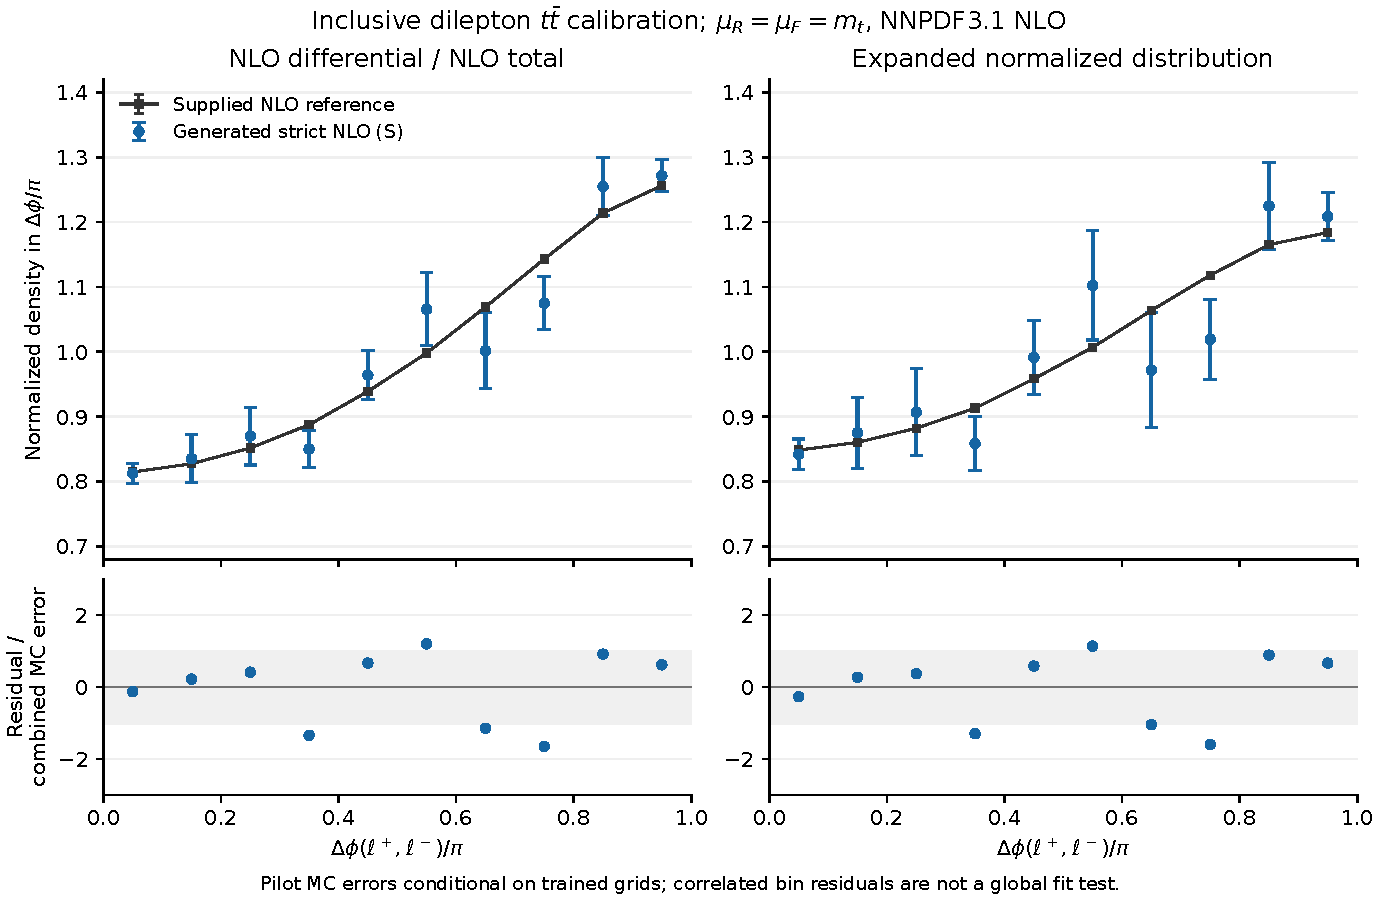
\includegraphics[width=\linewidth]{../figures/ttbar_reference_ref1901_v6.pdf}
\caption{Matched dilepton-$t\bar t$ validation against the normalized
angular distributions of Ref.~\cite{Behring2019}. The numerator scales
and width convention are those of the reference, rather than the dynamic
ttW benchmark. These conditional-error pilot comparisons test both
normalized-shape conventions; they do not establish percent-level
between-retraining coverage.}
\label{fig:ttbarvalidation}
\end{figure}

\subsection{Scale, current and mass checks}

Eight direct-scale comparisons test reweighting against independently
integrated physical scale choices. Their largest rate residual is 2.14
conditional Monte Carlo errors. Sixteen native-production/current versus
factorized-decay normalization comparisons have maximum absolute nominal
residual 2.19. The associated direct leptonic current receives only the
two top branching densities, with no additional associated-W branching
factor. The separate subtraction-scale check merits additional care:
an earlier uncut product comparison differed by 3.44 conditional errors,
whereas a freshly trained half-scale versus double-scale pair gives
$-0.84\pm4.09$ ab. These two pairs motivate monitoring retraining scatter;
they do not establish its coverage.

The generated narrow-W test keeps the weak couplings fixed, sets
$\Gamma_W=\epsilon\Gamma_W^{\rm ref}$, recomputes the matched top widths,
and uses the common fixed numerator scale $m_t+M_W/2$. Multiplying the
BW cross section once by $\epsilon^3$ removes the three inverse-width
factors. At $\epsilon=0.05$, the LO two-b ratios to the on-shell result
are $1.0028\pm0.0067$ for top BW and $1.0032\pm0.0063$ for all BW.
Using five independently retrained on-shell strict-NLO references gives
$0.9854\pm0.0321$ and $1.0139\pm0.0284$ for S. Only the on-shell reference
has a between-retraining error in this comparison; each BW control is
still a single conditional estimate. The shared reference is propagated
to both ratios. Several normalized tails remain unstable, in particular
the minimax distribution. Percent-level NLO narrow-W continuity is
therefore not established.

For massive decays, production amplitudes, flavour inputs and
production-owned subtraction sectors are checked against the massless
five-flavour export. The small-mass tests at $m_b=1$ and $0.1\GeV$ use
matched numerator masses and top widths in both on-shell and all-BW
samples. Among 320 populated nominal rate ratios the largest residual
is 2.66 conditional errors; one of 420 selected normalized-shape entries
reaches 3.34. One extreme integration split was excluded by the separately
documented protection used in that pilot campaign. Its retained-sample
errors omit selection bias. These tests bound the pilot sensitivity;
they do not certify the full-flavour massive or finite-W-width prediction.
